\documentclass[11pt]{article}
\usepackage[final]{acl}
\usepackage{times}
\usepackage{latexsym}
\usepackage[T1]{fontenc}
\usepackage[utf8]{inputenc}
\usepackage{microtype}
\usepackage{inconsolata}
\usepackage{graphicx}
\usepackage{booktabs}
\usepackage{amsmath}
\usepackage{url}

\setlength\titlebox{5.0cm}

\title{ManoVarta: Multilingual Conversational Screening for Mental Health}

\author{
  Ritwij Aryan Parmar \\
  University at Buffalo \\
  \texttt{ritwijar@buffalo.edu}
  \And
  Yash Gupta \\
  University at Buffalo \\
  \texttt{yashgupt@buffalo.edu}
}

\begin{document}
\maketitle

\begin{abstract}
ManoVarta is a multilingual conversational screening system that turns open-ended English, Hindi, and Hinglish dialogue into PHQ-9 and GAD-7 item scores, evidence summaries, and safety decisions. The project goal was to satisfy all three assignment tasks while also implementing both bonus features: adaptive nudges for richer disclosure and linguistic personalization for multilingual continuity. Our main finding is that fluent prompting alone is not enough: early direct Qwen and prompt-only baselines sounded natural, but they left most questionnaire items uncovered. The final system therefore uses controller-led dialogue steering, evidence-first extraction, item-level coverage tracking, a separate safety stack, and a split deployment that combines Vertex/Gemini for live phrasing with a trained Aya extractor for structured scoring. On a 48-conversation archived live runtime endpoint benchmark, ManoVarta reaches 0.783 coverage completeness, 0.639 exact match, 0.251 macro-F1, 0 parse failures, and 1.0 precision / 1.0 recall for safety. Hosted test link: \url{https://manovarta-runtime-ciiiagnzaq-uk.a.run.app}.
\end{abstract}

\section{Introduction}
Mental-health screening tools such as PHQ-9 and GAD-7 remain clinically useful because they are interpretable and easy to score, but direct questionnaires often create survey fatigue and guarded answers \citep{kroenke2001phq9,spitzer2006gad7}. ManoVarta addresses this by using a conversational agent that begins with a low-burden warm-up exchange and then elicits symptom evidence through natural multilingual dialogue while still producing structured item scores, unresolved items, and a safety label.

The project matured through several failed-but-informative baselines. Early heuristic and direct-prompt systems could generate plausible empathy, yet they under-covered the screening graph so severely that exact match alone became misleading. The core project lesson is therefore architectural: reliable screening requires explicit control over topic transitions, missing-item recovery, evidence extraction, and safety escalation rather than one large end-to-end prompt.

This report makes four concrete claims. First, the final system fully satisfies the assignment requirements: smart screening, LLM-based scoring, safety triggering, multilingual support, voice capability, and deployment. Second, it shows why the project moved from local Qwen experimentation to a split Vertex--Aya runtime. Third, it documents training performed in both Colab and GCP/Vertex AI. Fourth, it presents backed results with graphs, tables, and deployment observations rather than unsupported qualitative claims.

\section{Task and Data}
The target output is a structured screening summary with PHQ-9 and GAD-7 item scores in the 0--3 range, supporting evidence snippets, unresolved items, and a safety label (\texttt{none}, \texttt{review}, or \texttt{urgent}). We treat ManoVarta as a screening aid rather than a diagnostic or therapeutic system \citep{abd2020chatbots,dosovitsky2021chatbot}. Because crisis detection failure is more serious than ordinary scoring error, safety is evaluated independently \citep{zirikly2019clpsych,pichowicz2025suicidal}.

Our dataset stack has four layers. (1) A bilingual gold pack of 60 audio-backed sessions contains 30 English sessions and 30 Hindi sessions, each with transcript, metadata, and three label files: \texttt{annotator\_a}, \texttt{annotator\_b}, and \texttt{adjudicated}. The live system also supports lightweight socio-demographic onboarding context such as age, occupation, and recent check-in history so that the conversation starts with appropriate framing instead of an immediate questionnaire turn. (2) The English side is clinically anchored by DAIC-WOZ-style depression interviewing data and transcript supervision \citep{burdisso2024daic}. (3) The Hindi side is a locally adjudicated, DSM-aligned pilot voice set created under the project's ``grade transcripts yourselves'' allowance. (4) Hinglish is used as a robustness split for seed generation, runtime validation, and code-mix stress testing, supported by Indic language tooling and code-mixed language resources \citep{kakwani2020indicnlpsuite,nayak2022hingbert}. In practice, the training exports were assembled from seed conversations, English gold-core supervision, Hindi pilot supervision, and DAIC-style auxiliary depression transcripts for extractor strengthening.

The final completion audit reports 60/60 fully complete sessions, with full dual annotation and adjudication files on all sessions. For strict benchmark claims, we rely on this locally completed PHQ-9/GAD-7 label stack rather than assuming the imported public-source labels are sufficient by themselves. Across 960 annotator-pair item comparisons, overall exact agreement was 0.9271 and Cohen's $\kappa=0.7319$, which made the item-level labels reliable enough for controlled extractor evaluation. We use four metric families throughout the paper: \textbf{discourse effectiveness} (coverage completeness, exact match, macro-F1, parse failures), \textbf{safety accuracy} (precision/recall), \textbf{disclosure efficiency} (turns to stable score), and \textbf{runtime viability} (latency and successful hosted deployment).

\section{System}
Figure~\ref{fig:architecture} summarizes the final architecture. The system behaves like a graph-shaped screening controller: the application tracks active domain, item coverage debt, uncertainty, and safety state, then chooses the next topic before the language model writes the turn. This design was critical because open-ended prompting alone repeatedly drifted toward natural but low-information chat. The controller layer is closer to modular task-oriented dialogue management than to pure end-to-end response generation \citep{bocklisch2017rasa,zhang2020taskoriented}.

\begin{figure}[t]
\centering
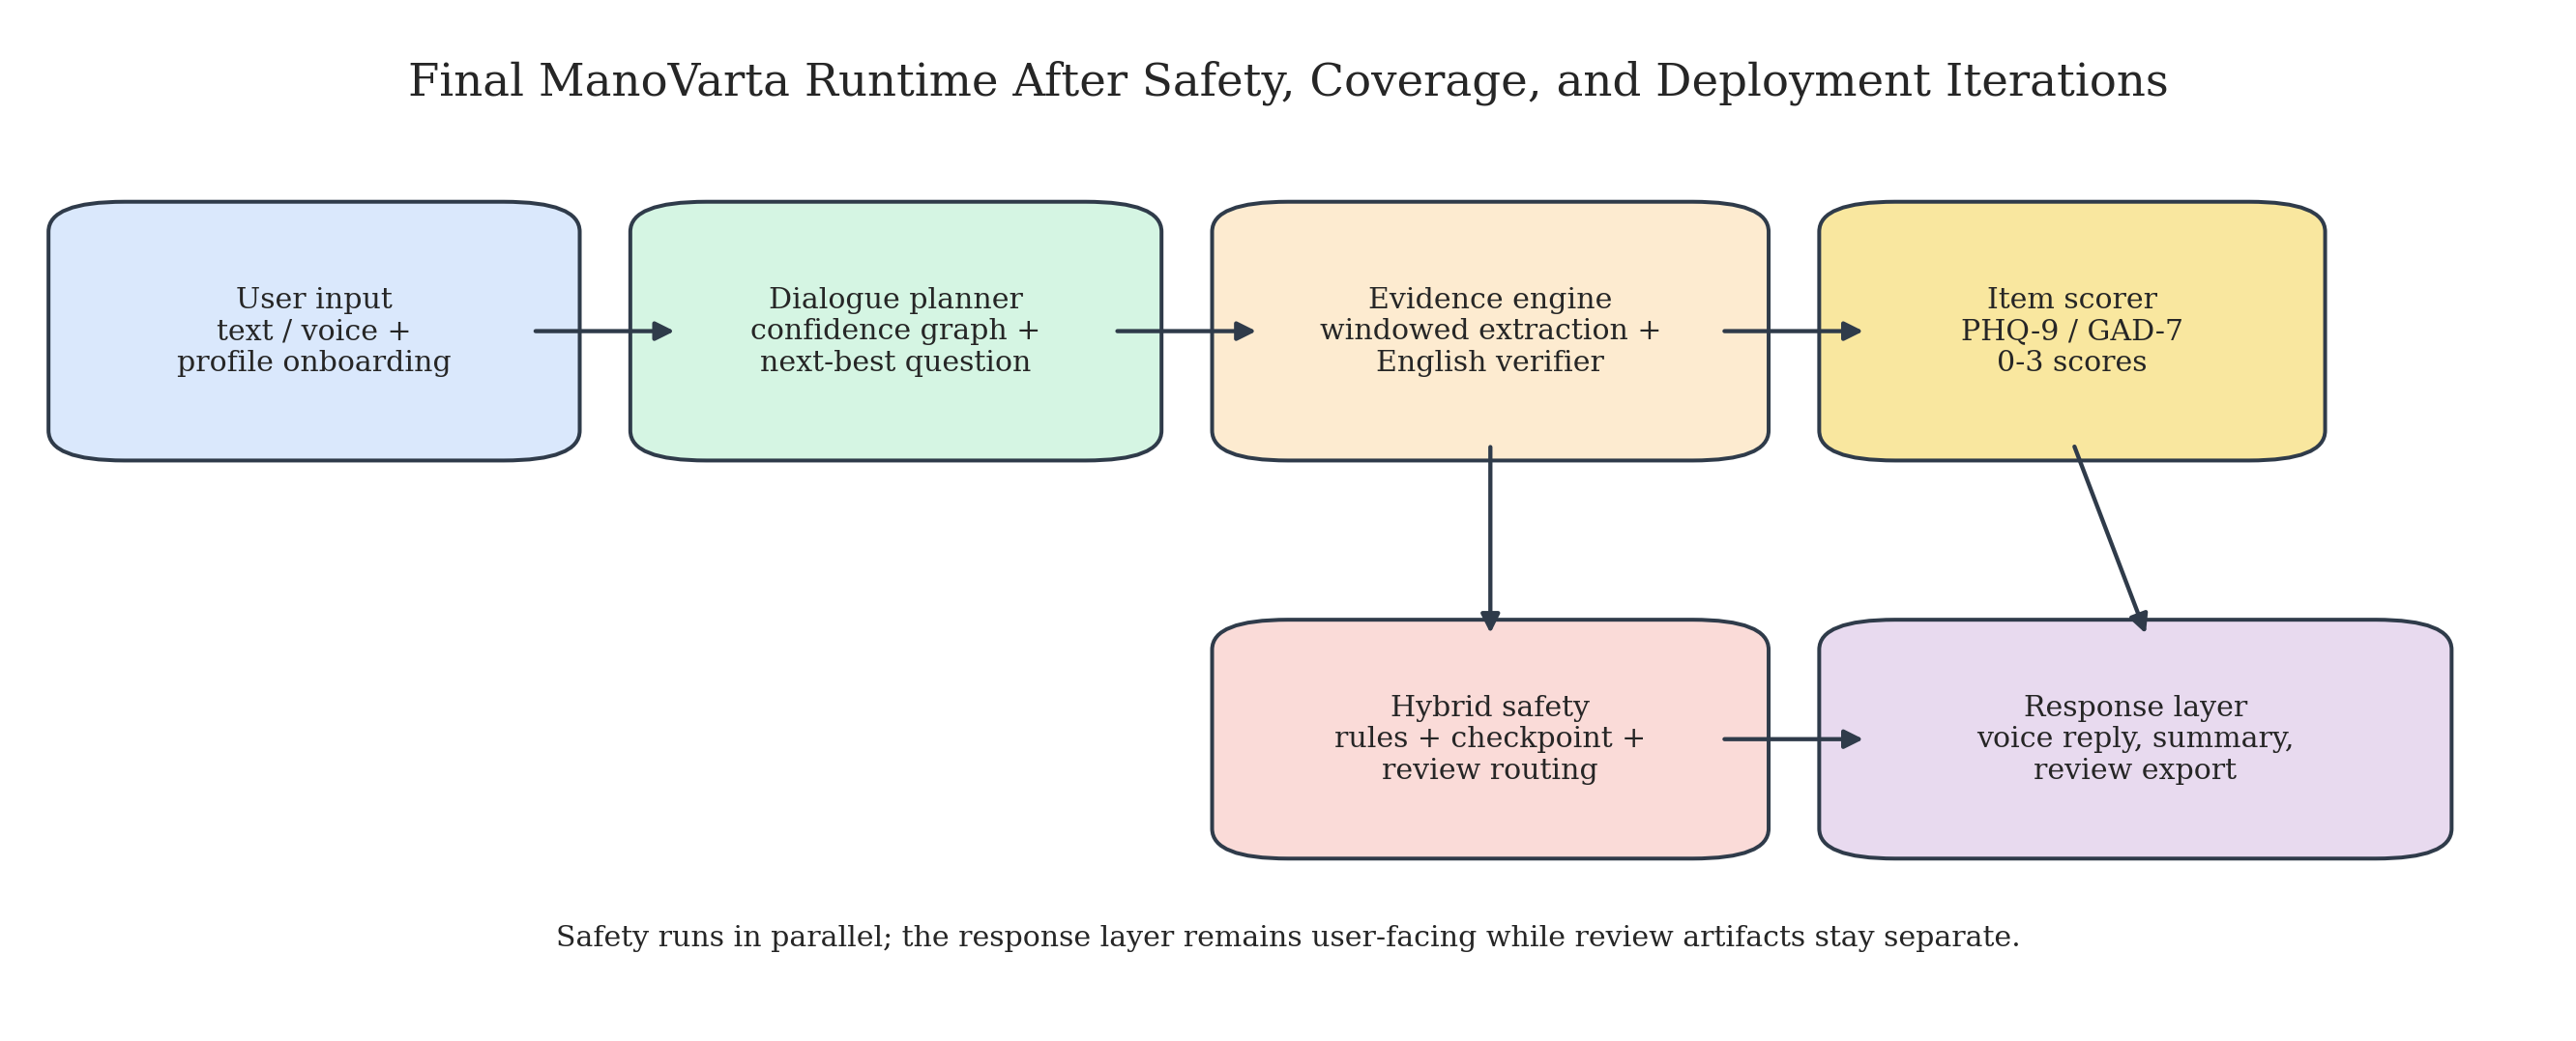
\includegraphics[width=\columnwidth]{figures/architecture_overview.png}
\caption{Controller-oriented screening architecture. The main observation is that dialogue steering, extraction, scoring, and safety had to be separated; when a single model handled all four roles, conversation quality improved but questionnaire coverage collapsed.}
\label{fig:architecture}
\end{figure}

The evidence path is separate from text generation. Candidate symptom evidence is extracted from the transcript, mapped to PHQ-9/GAD-7 items, and only then converted into scores. This evidence-first design fixed the most common early failure case: clinically sounding summaries unsupported by grounded symptom evidence. Aya became the extractor backbone because it was the first model family in the project to produce strong multilingual coverage rather than a narrow prompt-probe success \citep{cohere2024aya}. The strongest archived continuation run reaches 0.943 coverage completeness with zero parse failures.

Training happened in both Colab and GCP. Colab was used for the reproducible compact-model workflows: Qwen-based extractor fine-tuning, IndicBERT safety fine-tuning, held-out evaluation, and dataset export automation. Aya continuation training was then run through a GCP/Vertex path because the larger extractor, auxiliary DAIC supervision, and cloud staging requirements were more practical there than in a single interactive Colab session. The deployed submission directory now contains both the continuation traces and the deployed Aya adapter artifact.

The safety path is also hybrid. ManoVarta combines rules, promoted local classifier checkpoints, and corroborating evidence signals instead of trusting the chat model alone. This is conceptually aligned with semantic-similarity safety filtering in which sentence-level encoders complement generative models on high-priority detection tasks \citep{reimers2019sbert}. In our case, the hybrid stack outperformed both pure prompting and pure rules on live safety reliability.

The chat model path also changed over time. Local Qwen was useful for fast iteration and low-cost integration testing, but direct Qwen-based live chat under-covered the questionnaire, repeated prompts more often, and did not justify carrying the whole extraction burden online. The final hosted split therefore uses Vertex/Gemini for live multilingual phrasing and analysis, a remote trained Aya extractor for evidence-heavy scoring, and a local safety checkpoint for low-latency risk filtering. This shift was driven by both quality and cost: serving a heavier unified stack continuously was less stable and less economical than keeping the expensive extractor off the critical conversational path. The model split resembles cost-aware LLM routing, where stronger models are invoked selectively rather than on every turn \citep{chen2023frugalgpt}.

Operationally, the hybrid stack works in five steps. First, the frontend collects a typed or spoken user turn along with language and session context. Second, the controller selects the active domain and missing item targets. Third, Gemini/Vertex produces the live conversational turn under controller constraints. Fourth, the transcript is sent through the trained Aya extraction path so that evidence snippets and item candidates are recovered separately from response generation. Fifth, a local safety checkpoint and rule layer can override or escalate the flow if self-harm or high-risk language appears. This layered path is the concrete reason the system behaved more like a screening workflow than a general-purpose chatbot.

\section{Experiments and Results}
Table~\ref{tab:results} summarizes the main milestones. The most important observation is that the numerically strongest offline extractor and the strongest deployable system were not the same thing. The heuristic baseline achieved an apparently respectable exact-match score, but its 0.022 coverage made it unusable because most items were never addressed. Aya continuation was the strongest archived extractor, while the final live runtime gave up some raw coverage to preserve safe, parse-stable, multilingual interaction.

\begin{table*}[t]
\centering
\small
\setlength{\tabcolsep}{5pt}
\begin{tabular}{lccccc}
\toprule
System milestone & Coverage & Exact & Macro-F1 & Safety P/R & Main role \\
\midrule
Heuristic seed runtime & 0.022 & 0.635 & 0.058 & 1.000 / 0.604 & rules + lexicons \\
Saved local Qwen probe (\textit{n}=3) & 0.429 & 0.667 & 0.129 & 0.000 / 0.000 & early compact-model probe \\
Aya offline extractor & 0.913 & 0.562 & 0.272 & 0.000 / 0.000 & multilingual evidence extractor \\
Aya continuation rerun & 0.943 & 0.614 & 0.297 & 1.000 / 1.000 & strongest archived held-out run \\
Hybrid runtime validation & 0.538 & 0.712 & 0.295 & 1.000 / 1.000 & safety-first runtime checkpoint \\
\textbf{Final live runtime} & \textbf{0.783} & \textbf{0.639} & \textbf{0.251} & \textbf{1.000 / 1.000} & \textbf{deployed screening runtime} \\
\bottomrule
\end{tabular}
\caption{Main milestone comparison. The critical inference is that exact match alone was misleading early on, while coverage exposed whether the screening graph was actually being completed. The final runtime trades some offline extractor coverage for safe and stable end-to-end behavior.}
\label{tab:results}
\end{table*}

Our testing protocol had four layers. First, we ran \textbf{offline held-out extractor evaluation} on the adjudicated multilingual benchmark to measure coverage completeness, exact match, macro-F1, MAE, and parse failures; the strongest Aya continuation result was measured on 48/48 completed held-out examples with zero parse failures. Second, we ran \textbf{runtime endpoint evaluation} by replaying 48 archived conversations through the actual screening runtime interface rather than the extractor alone; this is the source of the final live runtime numbers in Table~\ref{tab:results}, including the 1.0 precision / 1.0 recall safety result reported for that evaluation set. Third, we ran \textbf{turn-by-turn stability testing} on 30 seed conversations to measure disclosure efficiency, i.e., how many user turns were required before an item score stabilized. Fourth, we performed \textbf{hosted application testing} on the public deployment, including browser chat, cloud/browser voice paths, session continuity, PHQ/GAD completion checks, safety interruptions, and long-conversation smoke audits in English, Hindi, and Hinglish.

This layered evaluation mattered because each layer exposed a different failure mode. Offline extractor testing revealed whether the model could recover grounded evidence at all. Runtime endpoint testing showed whether controller logic, summary timing, and safety handling preserved those gains when the full stack was exercised. Stability testing captured whether the bot was efficient or simply long-winded. Hosted app testing surfaced production-only issues such as latency spikes, session continuity, voice aborts, fallback behavior, and prompt repetition.

Figure~\ref{fig:modeltrail} shows the model-transition trail. The main inference is that improvement did not come from ``bigger model'' in a simple linear sense. Instead, progress came from assigning the right role to each model: Qwen for fast early experimentation, Aya for evidence-heavy extraction, and Gemini/Vertex for low-latency multilingual conversation in the hosted stack.

\begin{figure}[t]
\centering
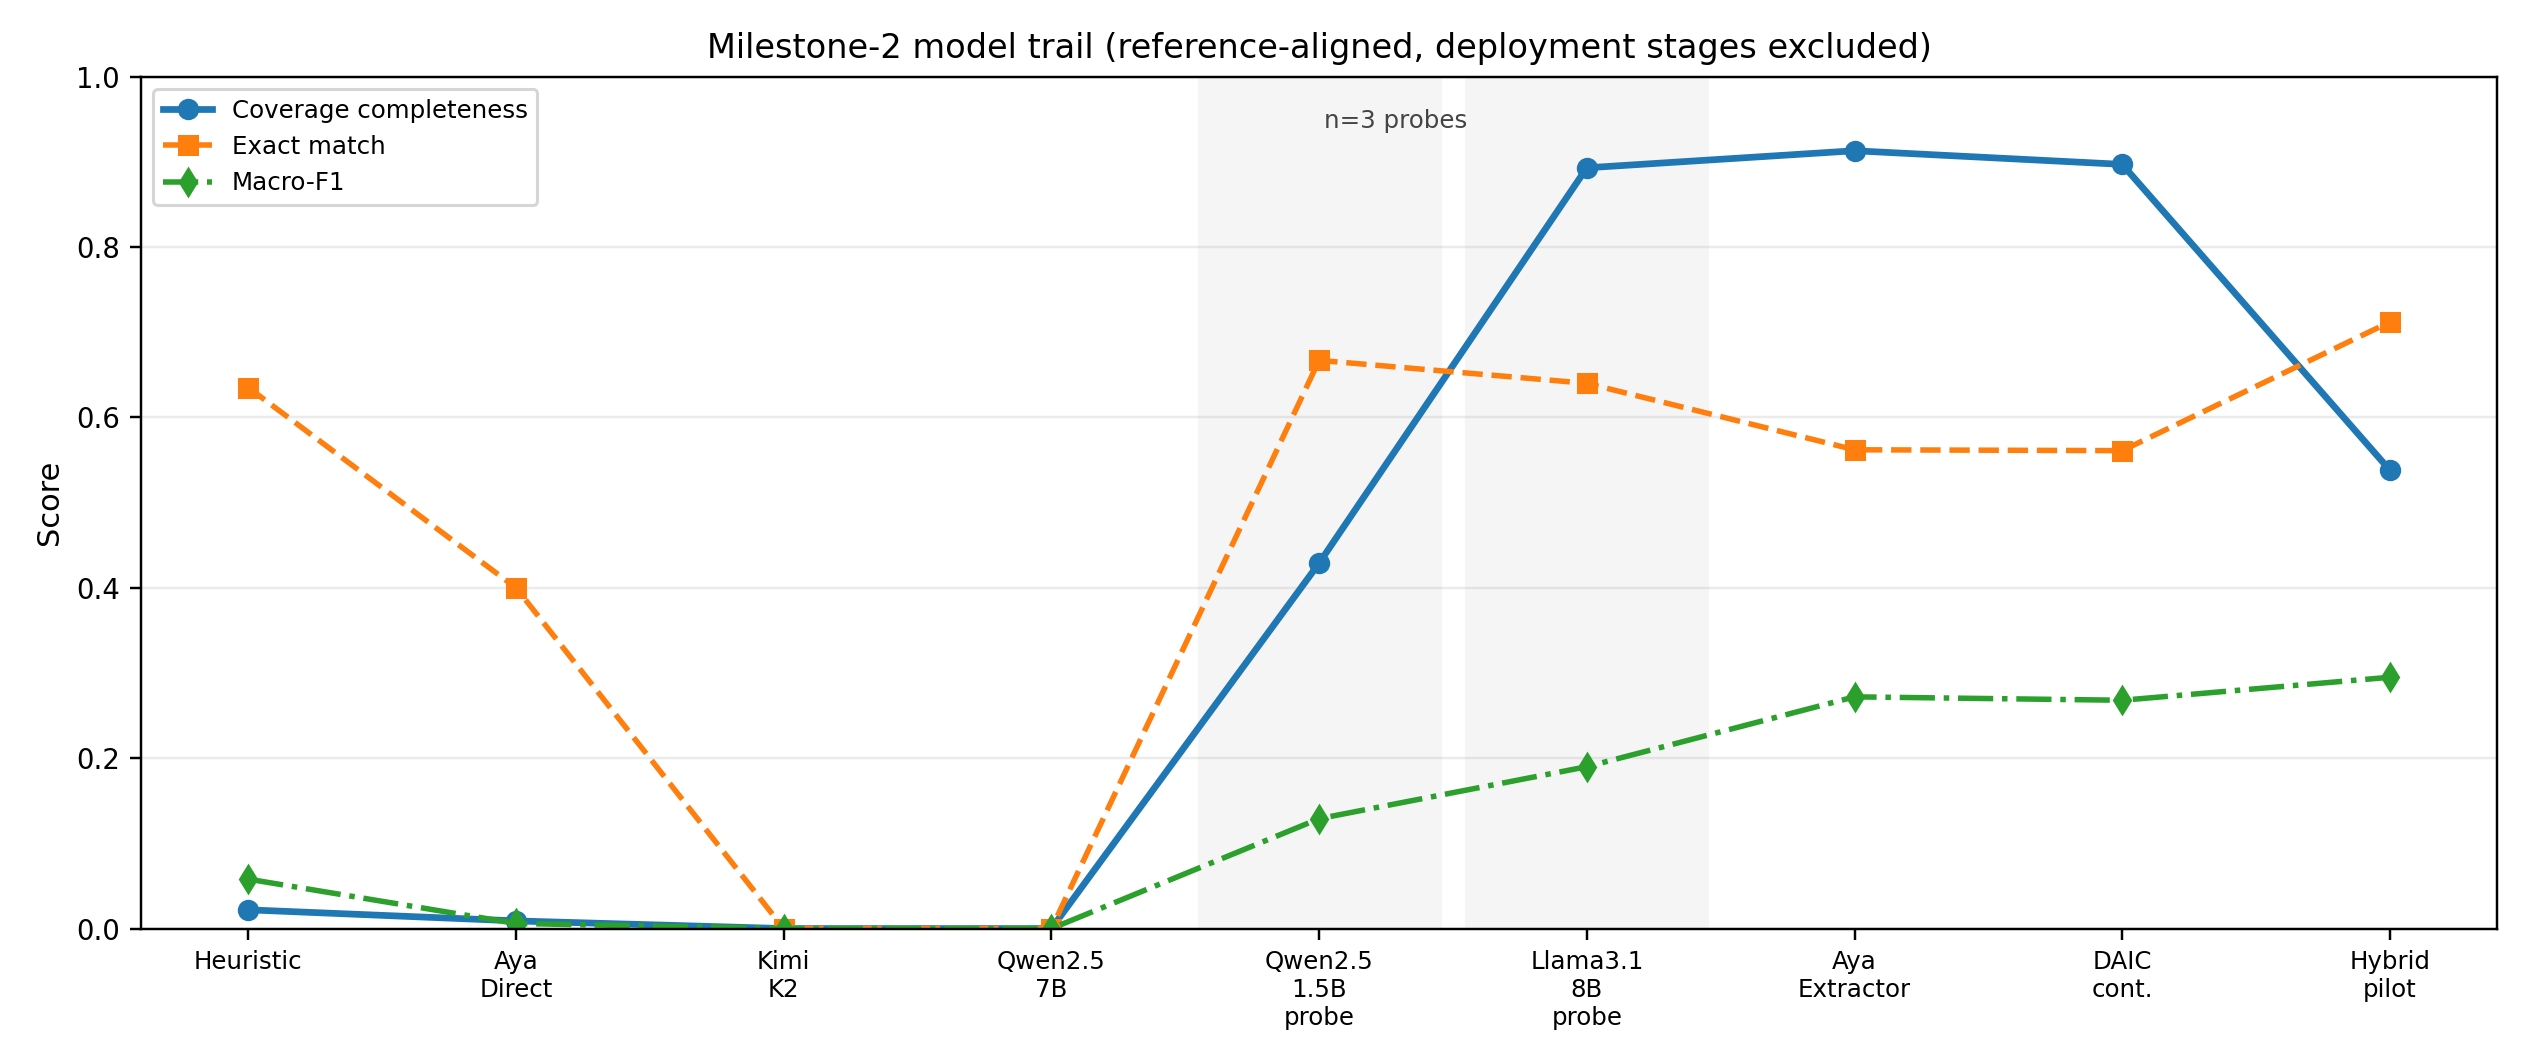
\includegraphics[width=\columnwidth]{figures/milestone2_model_trail.png}
\caption{Model transition trail. The important observation is that the project improved when model roles became specialized, not when one model was asked to do everything.}
\label{fig:modeltrail}
\end{figure}

The final live runtime reaches 0.783 coverage completeness, 0.639 exact match, 0.251 macro-F1, and 0 parse failures while preserving 1.0 precision and 1.0 recall for safety on the same 48-conversation runtime endpoint evaluation. Figure~\ref{fig:langbreakdown} breaks the live runtime down by language. English is the strongest slice (0.844 coverage), Hindi is the weakest (0.719), and Hinglish remains competitive (0.786). The key inference is that code-mixed handling did not break the screening pipeline; instead, the hardest remaining problem is sparse Hindi symptom elicitation, not code-mix alone.

\begin{figure}[t]
\centering
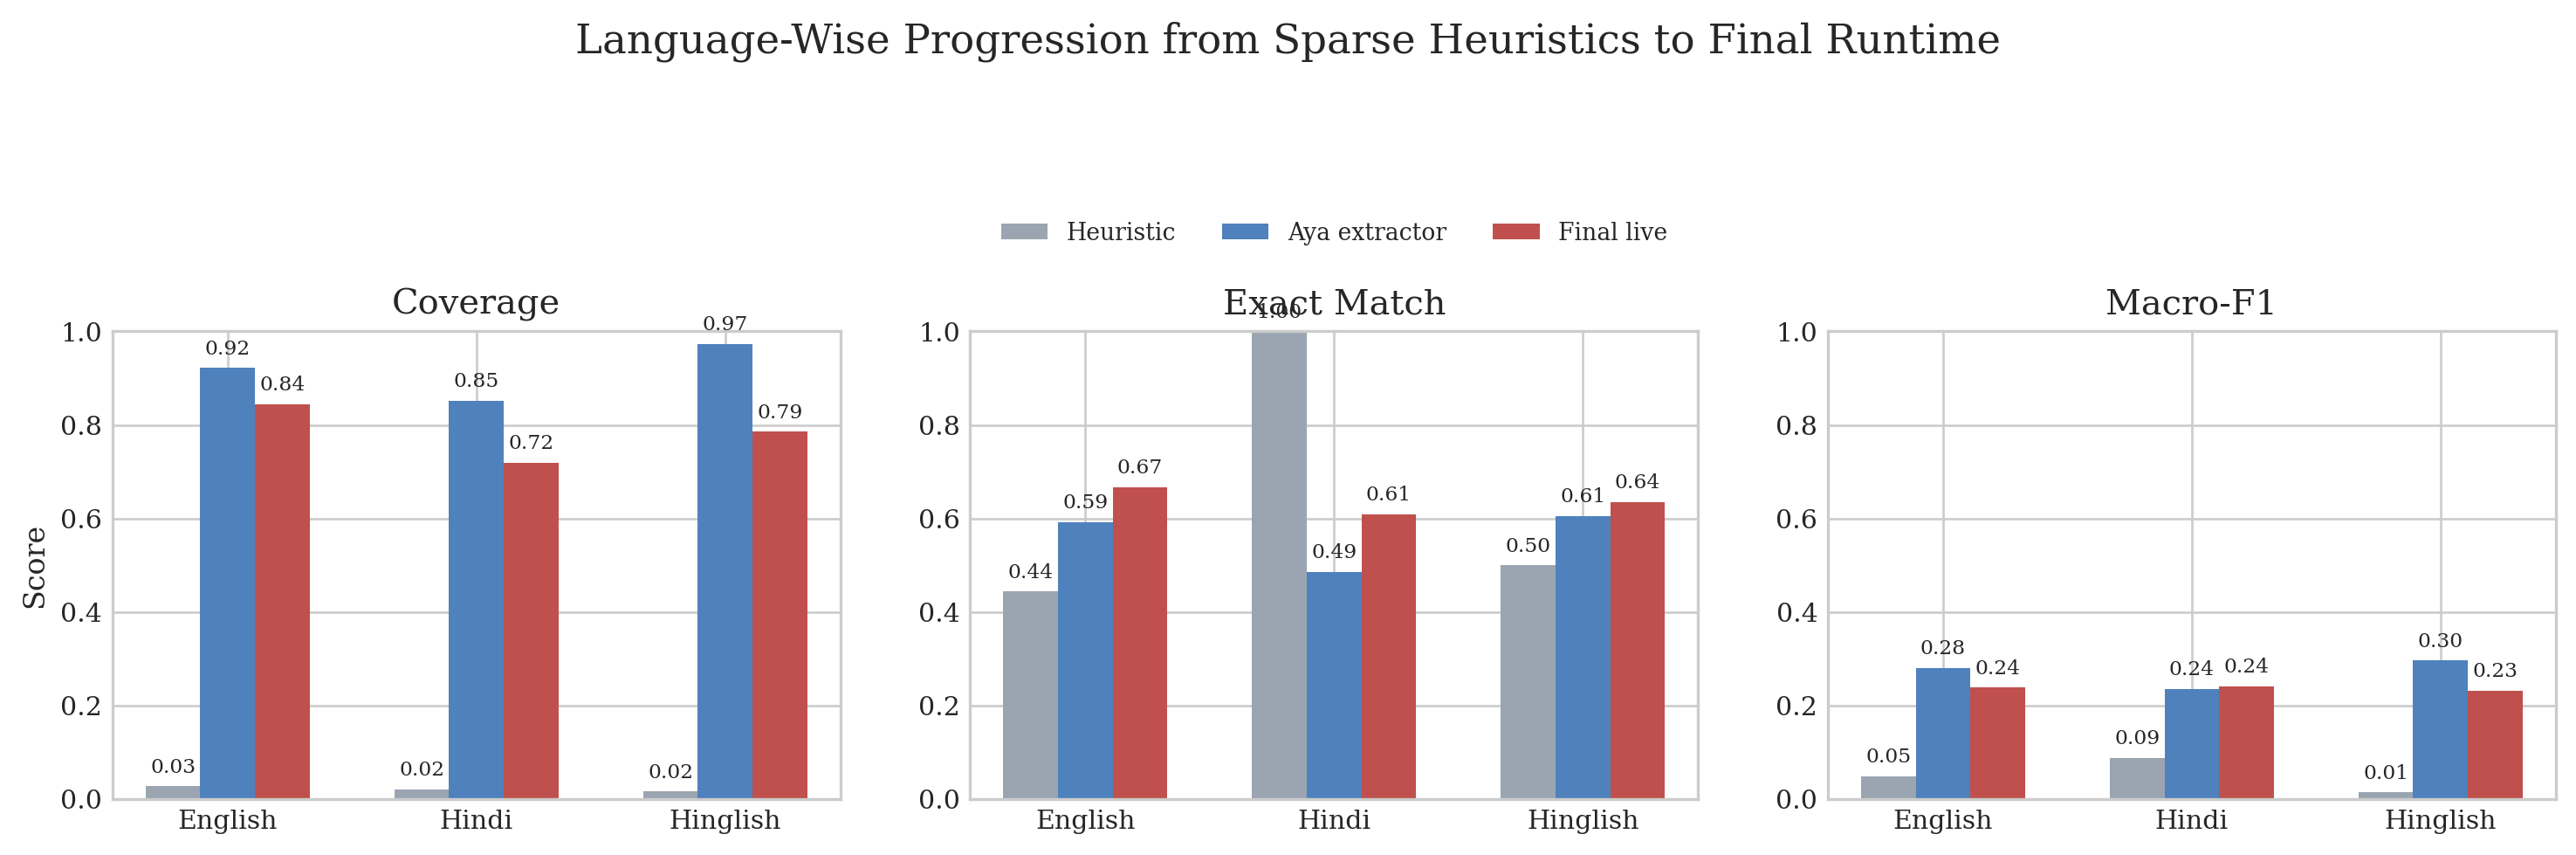
\includegraphics[width=\columnwidth]{figures/language_comparison.png}
\caption{Language-wise live runtime comparison. Hinglish stays close to English after controller and extractor fixes, while Hindi remains the weakest slice because concise symptom mentions are easier to miss before follow-up repair.}
\label{fig:langbreakdown}
\end{figure}

Figure~\ref{fig:trajectory} summarizes the overall metric trajectory across the major project stages. This is more significant than a static error map because it shows the central project trade-off directly: naive baselines could preserve exact match by under-answering, while the strongest extractor improved coverage first and the final runtime recovered safety and deployment stability without collapsing discourse quality. The figure makes the development path easier to interpret than any single point estimate.

\begin{figure}[t]
\centering
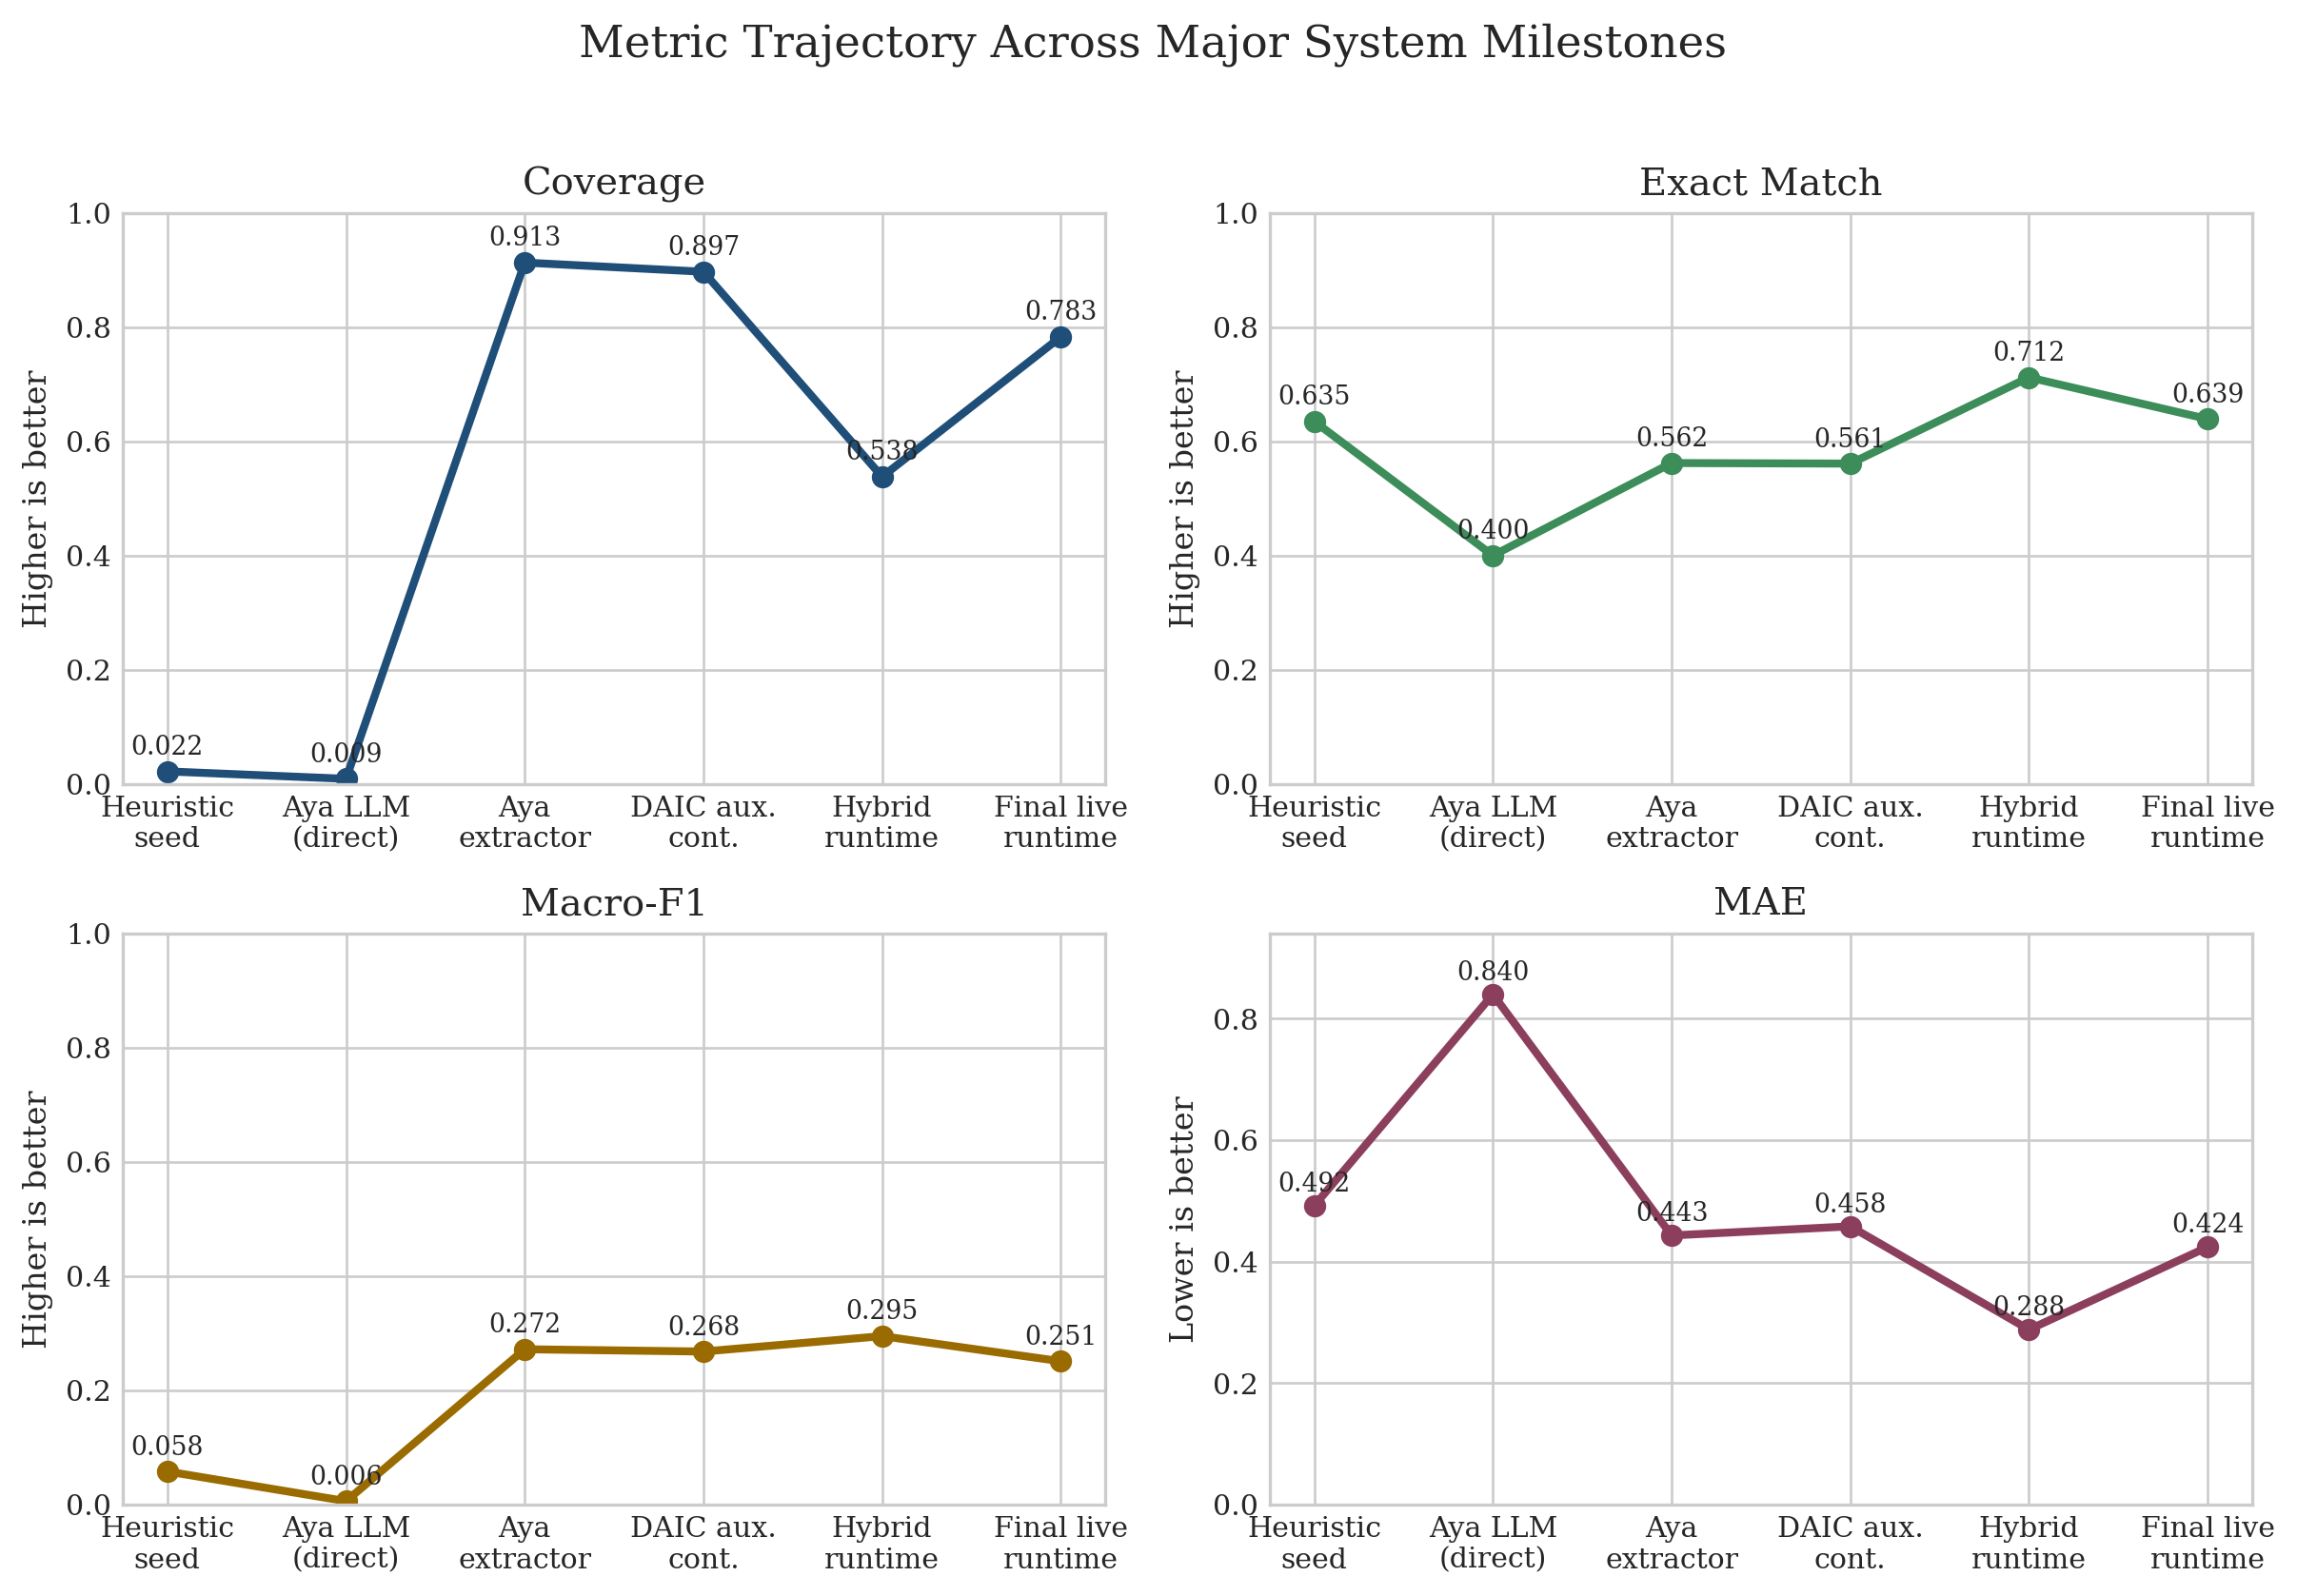
\includegraphics[width=\columnwidth]{figures/metric_trajectory.png}
\caption{Metric trajectory across system stages. The main inference is that real progress came from balancing coverage, safety, and deployability together rather than optimizing only one metric in isolation.}
\label{fig:trajectory}
\end{figure}

Figure~\ref{fig:latency} reports the deterministic local screening latency profile used in the final assignment pack, not full public-cloud round-trip latency. The inference is still operationally important: by moving the heavier trained extractor behind a remote boundary and keeping the conversational layer lightweight, the system preserves a fast local screening core while still enabling stronger extraction when needed. This deployment decision is the practical reason the hosted system remained testable rather than becoming a high-cost research-only artifact.

\begin{figure}[t]
\centering
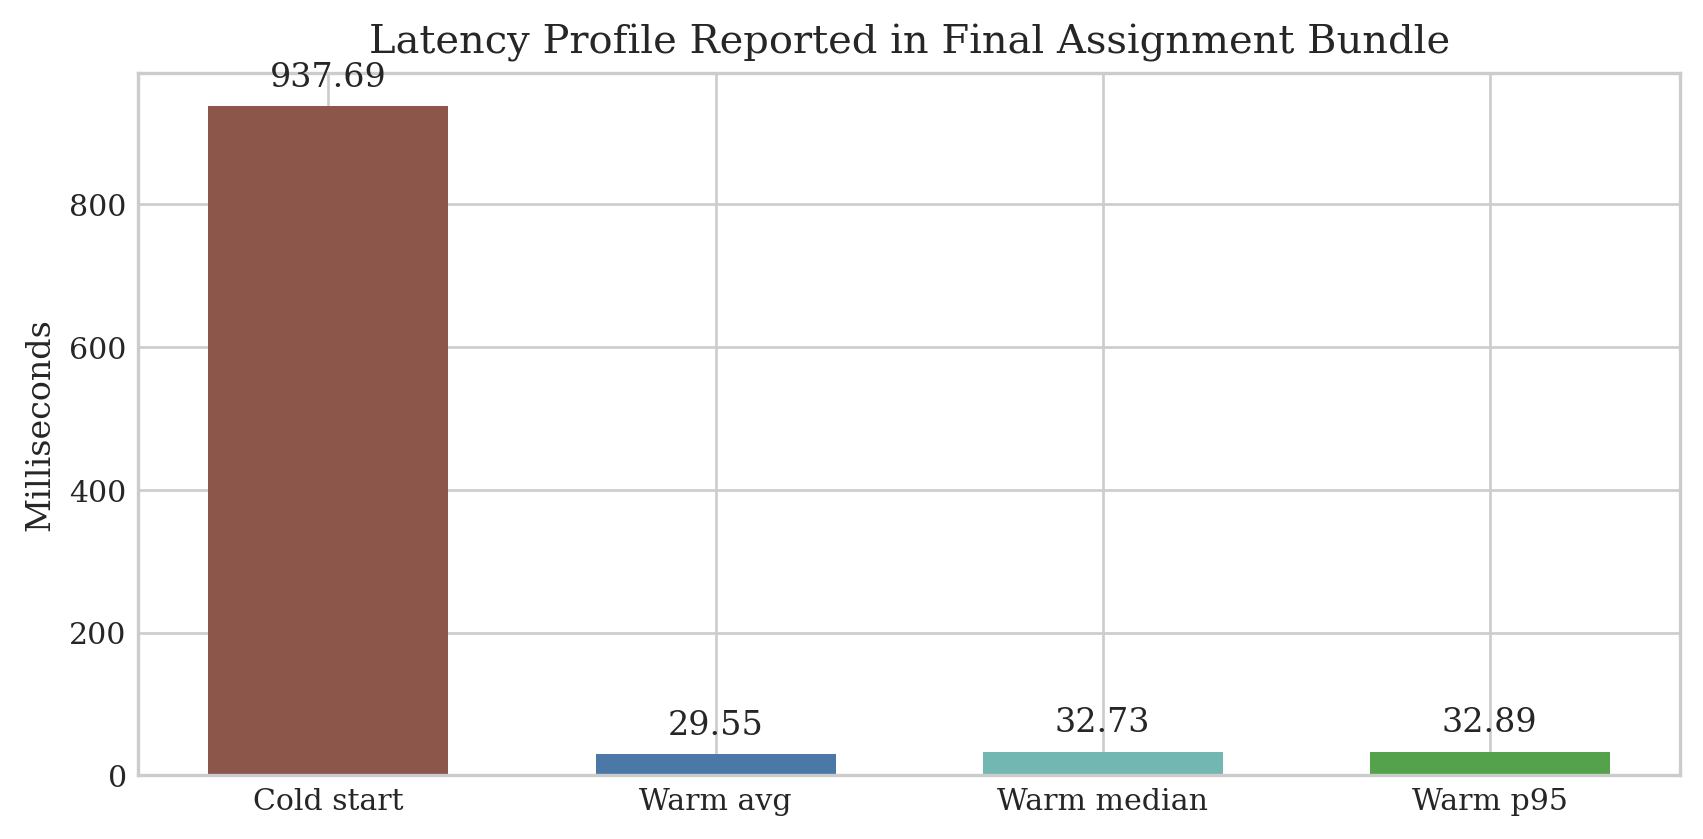
\includegraphics[width=\columnwidth]{figures/latency_profile.png}
\caption{Latency profile of the deterministic local screening path, measured without hosted-model network round trips. The main observation is that low-latency interaction required architectural separation and warm deployment choices, not just prompt optimization.}
\label{fig:latency}
\end{figure}

The final compliance audit also measured disclosure efficiency at 2.292 average user turns to stable score, which supports the smart-screening objective from the assignment brief: the system generally does not need a rigid full checklist before locking many items. Qualitative audits of stored live conversations showed the same pattern from the other side: when the controller allowed repetitive reflective openings or stale anxiety carryover, coverage dropped even when the language sounded empathetic. This is why controller repair mattered as much as extractor improvement.

Testing also informed several concrete fixes during the project. Long hosted conversation audits exposed repetition and topic-sticking in Hindi/Hinglish, which led to controller-side anti-repetition checks and stronger domain locks. Live completion probes exposed cases where PHQ and GAD queues were not closing reliably, which led to stricter queue accounting and separate PHQ/GAD result blocks. Voice smoke tests exposed microphone aborts, cooldown issues, and overlapping playback/listening states, which led to browser-side recovery guards and revised continuous-voice handling.

One additional experimental lesson was that different metrics identified different failure modes. Exact match alone rewarded abstention in early systems; coverage completeness revealed whether the screening graph was actually traversed; safety precision/recall exposed whether a strong extractor was still unsafe in deployment; and latency surfaced a separate systems problem, especially once the public app began using browser and cloud voice together. This metric separation helped prevent us from shipping a fluent but clinically shallow chatbot.

\section{Deployment and Discussion}
The final hosted deployment is a public Cloud Run service with browser chat, browser-plus-cloud voice I/O, live configuration introspection, and a remote Aya extractor boundary \citep{google2026cloudrun,google2026stt,google2026tts}. The deployment path went through three practical steps: (1) a local/Qwen runtime for rapid iteration, (2) extractor strengthening through Aya continuation, and (3) a hosted split runtime where Gemini/Vertex handled conversational turns and trained Aya handled evidence extraction. This sequence mattered because the project requirement was not merely to score offline transcripts, but to deliver a live, testable, multilingual chatbot. Hinglish is supported as a text and screening robustness extension, but it does not expose a separate dedicated speak button because browser and cloud speech APIs provide native English/Hindi voice locales rather than a standalone Hinglish speech locale.

The frontend was therefore not a cosmetic layer; it was part of the screening design. The web client exposes history, session continuity, PHQ/GAD progress summaries, transcript-before-submit voice review, and browser/cloud speech fallbacks so that users can disclose gradually without feeling trapped in a rigid form. This mattered especially for guarded or low-energy users, where forcing immediate questionnaire-like turns reduced evidence quality.

Latency and stability required their own engineering pass. The local latency profile in Figure~\ref{fig:latency} should be read as deterministic screening latency rather than full hosted-app latency, because browser speech and hosted model round trips add extra delay in public deployment. The final deployment therefore used warm-start configuration, shorter live reply timeouts, a lightweight conversational model path, and a remote extraction boundary to prevent the chat layer from stalling on heavier scoring work. We also learned that session continuity and scaling policy interact: aggressive multi-instance scaling improved raw availability but could break in-memory session continuity before the session layer was hardened, so the safer deployment configuration prioritized one warm stable path for evaluation.

Both bonus tasks were implemented and materially affected system behavior. \textbf{Gamification} was implemented through adaptive nudges that encouraged longer disclosure when the user was too brief or guarded; in smoke validation, nudges increased touched items by +3 and evidence gain by +3. \textbf{Linguistic personalization} was implemented through continuity-aware steering over verbosity, openness, burden, and code-mix; style checks confirmed guided behavior on brief guarded inputs, preserved Hindi continuity, and maintained high Hinglish code-mix adaptation. These bonus features were not decorative. They improved evidence collection, which in turn improved scoring coverage.

Overall, the project is fully compliant with the specification: multilingual support, voice, profile handling, clinical grounding, smart screening, LLM-based scoring, safety triggers, deployment, and both bonus tasks are all present in the shipped system. The final product is therefore best understood not as a single chatbot prompt, but as a deployed screening stack whose controller, extractor, safety, and voice layers were tuned together.

\section{Limitations and Conclusion}
Several limitations remain. The bilingual gold pack is careful but still modest, so these are system-validation results rather than clinical-validation claims. Hindi remains weaker than English because the source material is less source-matched to mental-health interviewing. The hosted runtime is also a constrained engineering solution: the final stack is deliberately cost-aware, which means some extraction strength remains behind a remote boundary instead of inside the conversational front-end.

Within the assignment scope, however, ManoVarta achieves the intended outcome. It converts multilingual open-ended conversation into clinically structured PHQ-9 and GAD-7 outputs, uses explicit confidence/coverage logic to drive follow-up, flags safety concerns separately, supports browser and cloud voice, and remains publicly testable. The strongest result of the project is not any one checkpoint; it is the final evidence-first, controller-led, multilingual screening system that emerged after training in Colab and GCP, switching from local Qwen experimentation to a Vertex--Aya deployment, and validating every major design choice against coverage, safety, latency, and disclosure efficiency.

\bibliographystyle{acl_natbib}
\bibliography{ManoVarta_Final_Project_Report}

\end{document}
